\section{Coordinate curvilinee e coordinate polari nel piano}
%---------------------------------------------------------------------------
In moti casi in fisica risulta particolarmente conveniente utilizzare 
tipologie diverse di coordinate, rispetto a quelle cartesiane. Due di queste sono le coordinate curvilinee e quelle polari.\\
Le coordinate cartesiane identificano la posizione di un punto materiale 
mediante tre coordinate, corrispondenti alla proiezione del punto lungo gli assi cartesiani. Utilizzando i versori canonici $\hat\imath$, $\hat\jmath$ e $\hat k$ possiamo scrivere:
\begin{equation}
    \vec x = \sx x, y, z\dx = x\hat\imath + y\hat\jmath + z\hat k\seg
    \vec v = \dot x\hat\imath +\dot y\hat\jmath +\dot z\hat k\quad\quad
    \vec a = \ddot x\hat\imath +\ddot y\hat\jmath +\ddot z\hat k
\label{eq:Cartesian}
\end{equation}
Le coordinate curvilinee identificano come posizione, la distanza effettivamente percorsa dal punto materiale, e utilizzano come direzioni principali quella tangente $(\hat\tau)$ e quella normale $(\hat n)$.\\

\begin{figure}[htbp]
    \begin{minipage}[b]{0.47\textwidth}
        \centering
            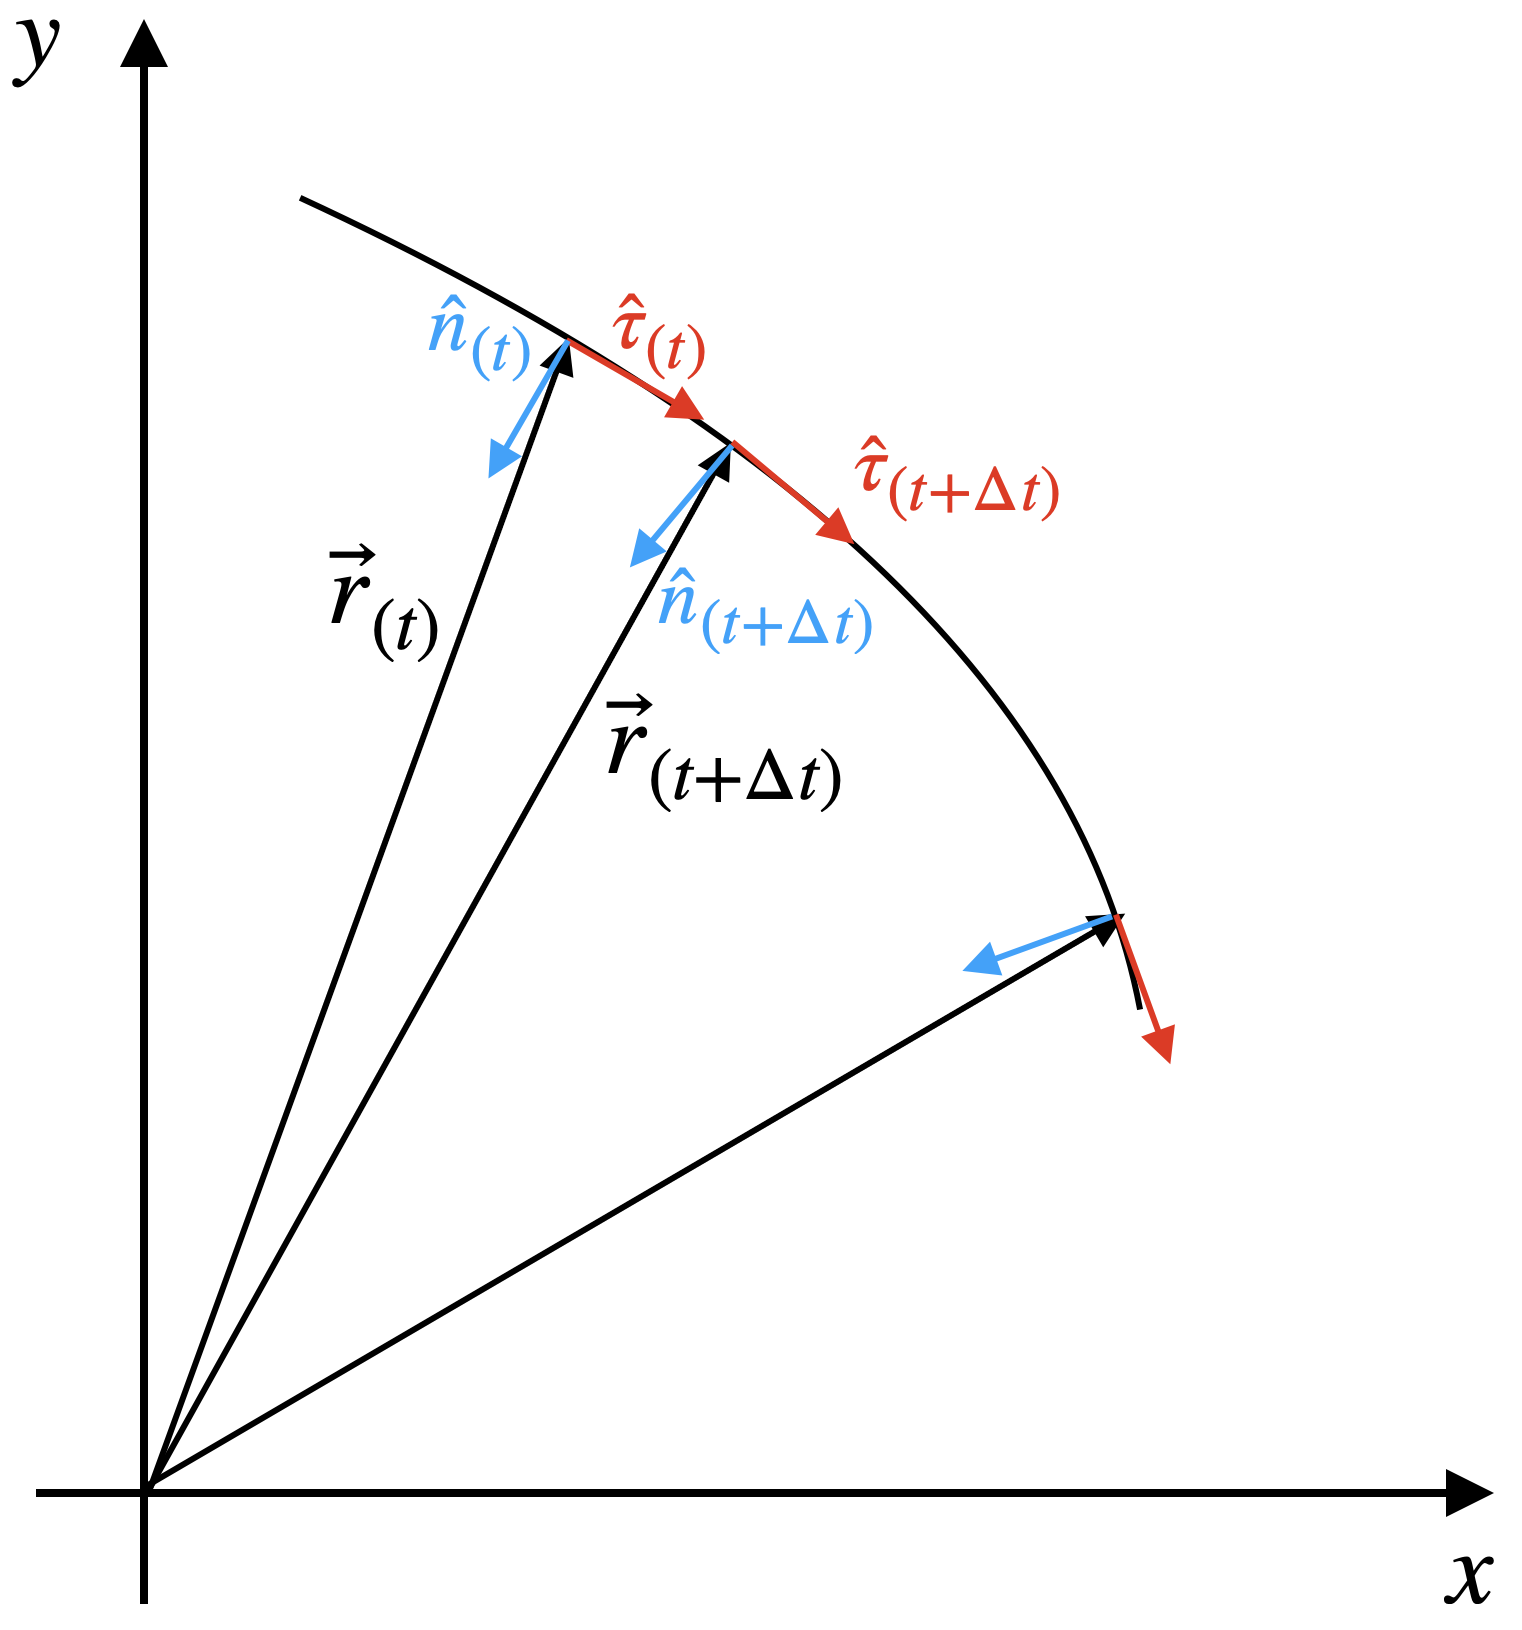
\includegraphics[width=7cm]{images/coordcurv.png}
            \caption{Rappresentazione dei versori tangente e normale lungo un tratto di curva.}
    \label{fig:curvilines}
    \end{minipage}
    \hfill
    \begin{minipage}[b]{0.47\textwidth}
        \centering
            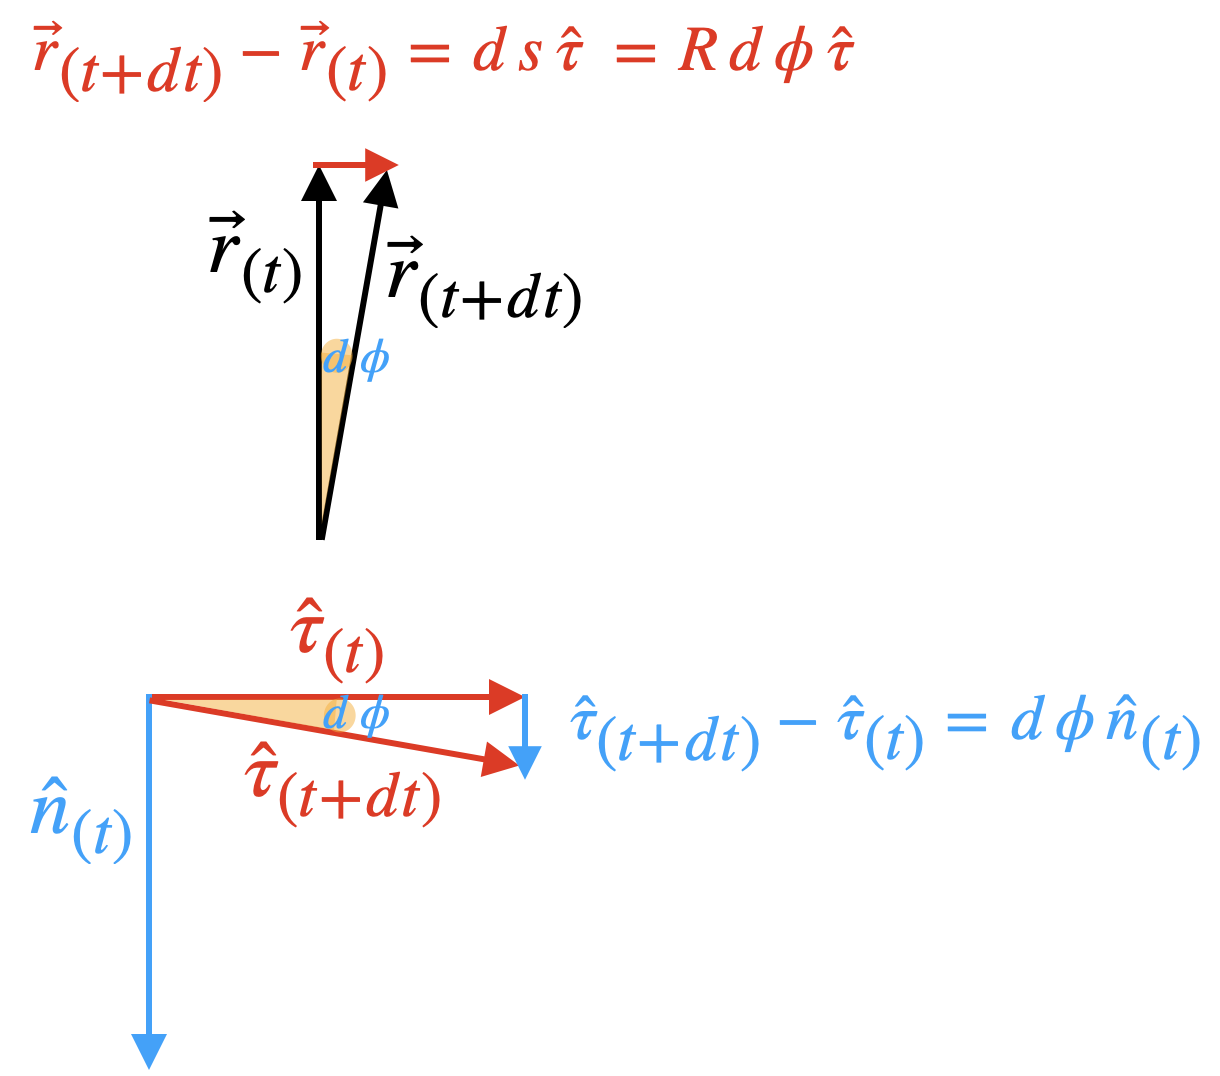
\includegraphics[width=7cm]{images/drdtau.png}
            \caption{Rappresentazione grafica della variazione infinitesima del vettore $\vec r$ e del versore $\hat\tau$.}
    \label{fig:drdtau}
    \end{minipage}
    \hfill
\end{figure}

\begin{equation}
    d\vec x = ds\hat\tau\seg \vec v = \dot s \hat\tau = v\hat\tau\seg
    \vec a = \ddot s\hat\tau + \dot s\dot\phi\hat n
\end{equation}
\begin{equation}
    \dot\phi = \frac{d\phi}{ds}\dot s = \dot s \frac{d\phi}{Rd\phi} =
    \frac{v}{R}
\label{eq:omega}
\end{equation}
\begin{equation}
    \boxed{\vec v = v\hat\tau}\quad\quad \boxed{\vec a =
    \dot v \hat\tau + \frac{v^2}{R}\hat n = a_t\hat\tau + a_n\hat n}
\label{eq:curvilines}
\end{equation}                                                                                                                                                                                                                                                                                                                                                                                                                                                                                                                                                                                                                                                                                                                                                                                                                                                                                                                                                                                                                                                                                                                                                                                                                                                                                                                                                                                                                                                                                                                                                                                                                                                                                                                                                                                                                                                                                                                                                                                                                                                                                                                                                                                                                                                                                                                                                                                                                                                                                                                                                                                                                                                                                                                                                                                                                                                                                                                                                                                                                                                                                                                                                                                                                                                                                                                                                                                                                                                                                                                                                                                                                                                                                                                                                                                                                                                                                                                                                                                                                                                                                                                                                                                                                                                                                                                                                                                                                                                                                                                                                                                                                                                                                                                                                                                                                                                                                                                                                                                                                                                                                                                                                                                                                                                                                                                                                                                                                                                                                                                                                                                                                                                                                                                                                                                                                                                                                                                                                                                                                                                                                                                                                                                                                                                                                                                                                                                                                                                                                                                                                                                                                                                                                                                             
L'accelerazione in coordinate curvilinee ha due componenti, una tangente ed una normale o centripeta. La velocità invece è sempre tangente alla traiettoria percorsa.\\
Per quanto riguarda invece le coordinate polari, si scelgono come direzioni principali quella radiale $(\hat r)$ e quella trasversa $(\hat\phi)$.

\begin{figure}[htbp]
    \centering
        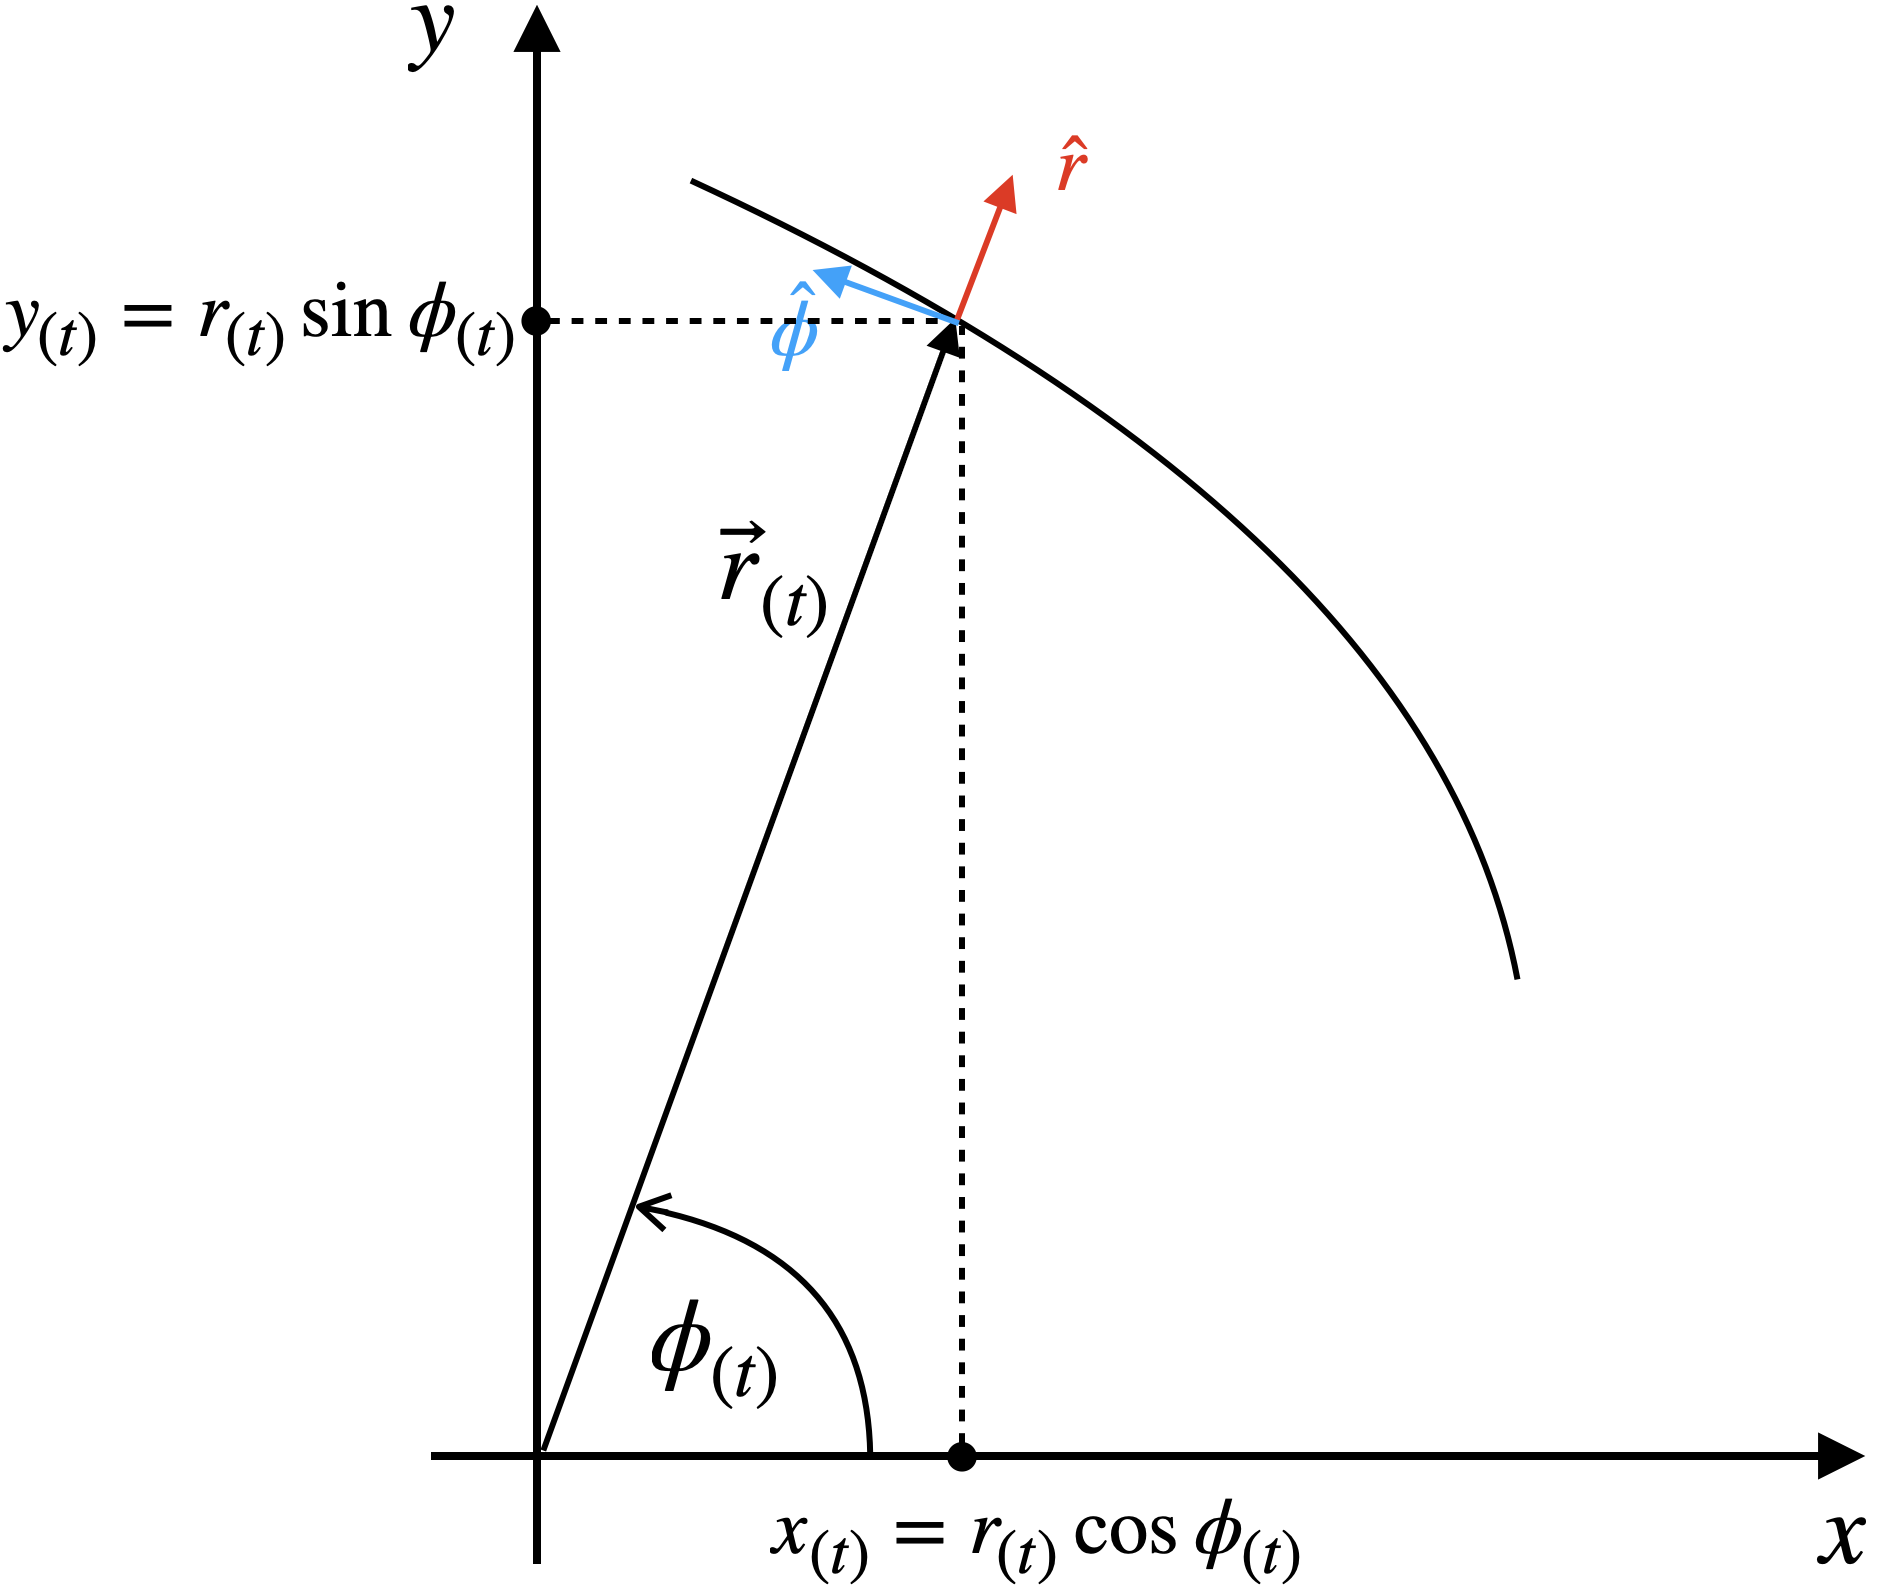
\includegraphics[width=7cm]{images/coordpol.png}
        \caption{Rappresentazione dei versori tangente e normale lungo un tratto di curva.}
\label{fig:polaris}
\end{figure}

\begin{equation}
    \boxed{\vec x = r\hat r} \seg \boxed{\vec v = \dot r \hat r +
    r\dot\phi\hat\phi}
\label{eq:polaris_xv}
\end{equation}
Per ottenere l'espressione dell'accelerazione in coordinate polari è
necessario svolgere alcuni calcoli.
\begin{equation}
    \vec a = \frac{d\vec v}{dt} = \frac{d}{dt}\sx \dot r \hat r +
    r\dot\phi\hat\phi \dx = \ddot r\hat r + \dot r\frac{d\hat r}{dt} +
    \dot r \dot \phi \hat\phi + r\ddot\phi\hat\phi + r\dot\phi\frac{d\hat \phi}{dt}
\end{equation}
\begin{equation}
    \frac{d\hat r}{dt} = \dot\phi\hat\phi\quad\quad\quad
    \frac{d\hat \phi}{dt} = -\dot\phi\hat r
\end{equation}
\begin{equation}
    \vec a = \sx \ddot r - r\dot\phi^2\dx\hat r + \sx 2\dot r\dot\phi +
    r\ddot\phi\dx\hat\phi
\end{equation}
$$\Downarrow$$
\begin{equation}
    \boxed{\vec a = \sx \ddot r - r\dot\phi^2\dx\hat r +
    \left[\frac{1}{r}\frac{d}{dt} \sx r^2\dot\phi\dx\right]\hat\phi =
    a_r\hat r + a_{\phi}\hat\phi}
\label{eq:polaris_a}
\end{equation}